\documentclass[a4paper]{article}

\usepackage[utf8]{inputenc}
\usepackage[spanish]{babel}
\usepackage{graphics}
\usepackage{caption}
\usepackage{subcaption}
\usepackage[demo]{graphicx}
\usepackage{enumitem}
\usepackage{longtable}
\usepackage{listings}
\usepackage{listingsutf8}
\usepackage{framed}
\usepackage{float}
\usepackage{hyperref}
\usepackage{amsmath}

\begin{document}

\begin{titlepage}

\begin{center}
\vspace*{1.5in}
\vspace*{-1in}
\begin{figure}[htb]
\begin{center}

\includegraphics[width=8cm]{logoUZ.png}
\end{center}
\end{figure}

\vspace*{0.3in}

Universidad de Zaragoza \\

\vspace*{0.3in}

\begin{large}
VIDEOJUEGOS\\
\end{large}
\vspace*{0.2in}
\begin{Large}
\textbf{Super Bomberman} \\
\end{Large}
\vspace*{0.3in}
\begin{large}
\end{large}
\vspace*{0.1in}
\rule{80mm}{0.1mm}\\
\vspace*{0.1in}
\begin{large}
Hecho por: \\
Jaime Ruiz-Borau Vizárraga (546751) \\
Patricia Lázaro Tello (554309) \\

\end{large}
\end{center}

\end{titlepage}
\tableofcontents

\newpage
\section{Descripción del videojuego realizado}
\paragraph{}Como se describe en el título de la memoria, el videojuego clásico elegido para la elaboración de un clon es el \textbf{Bomberman}. Dada la elevada similitud de mecánica, enemigos y objetivos entre las distintas entregas de Bomberman, se optó por implementar la mecánica del \textbf{primer Bomberman} que salió al mercado. Sin embargo, los sprites y las imágenes empleadas para el juego son de entregas de Bomberman posteriores.
\vspace*{0.2in}
\begin{figure}[H]
	\centering
	\begin{minipage}[b]{0.4\textwidth}
		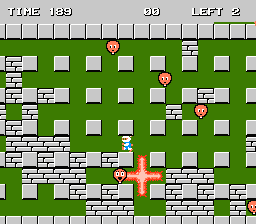
\includegraphics[width=\textwidth]{primerBomberman.png}
		\caption{Bomberman clásico}
	\end{minipage}
	\hfill
	\begin{minipage}[b]{0.4\textwidth}
		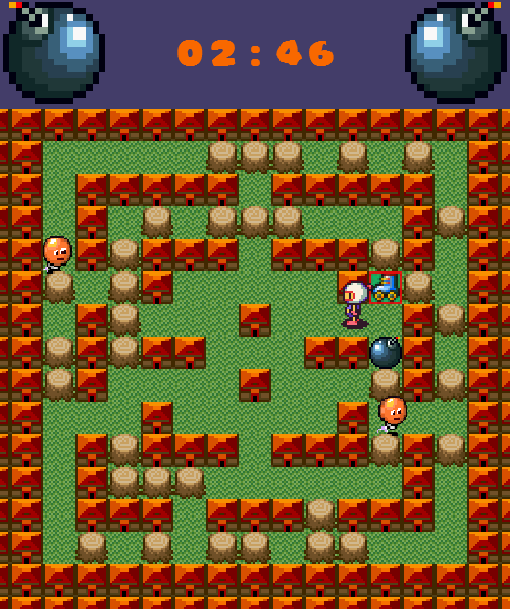
\includegraphics[width=\textwidth]{bomberman.png}
		\caption{Clon desarrollado}
	\end{minipage}
	\label{fig:primerBomberman}
\end{figure}
La única diferencia con el original es que la puntuación no se muestra hasta el final de la partida. También se ha implementado un menú con opciones para regular el volumen de la música del juego y la posibilidad de configurar los controles del juego.
\newpage
\section{Detalles de la implementación en 2D}
\paragraph{}Para el juego en 2D se implementó un motor gráfico basado en un hilo principal renderizando frames a razón de 60 por segundo, mostrando los distintos sprites del juego utilizando las funciones estándar de Java para mostrar gráficos por pantalla.
\paragraph{}El juego actualmente tiene 10 niveles generados aleatoriamente: posee unos mapas predefinidos de bloques no destruibles y dispone de forma aleatoria los enemigos y los bloques destruibles. Dichos bloques soltarán también de forma aleatoria los \textit{power-ups} mencionados anteriormente. Se obtienen puntos por destruir enemigos, por destruir bloques y por terminar niveles, y al terminar la partida, ya sea por acabar los 10 niveles o por morir a manos de un enemigo o una bomba, se muestra la tabla de mejores puntuaciones junto a la puntuación de dicha partida.
\begin{figure}[H]
	\centering
	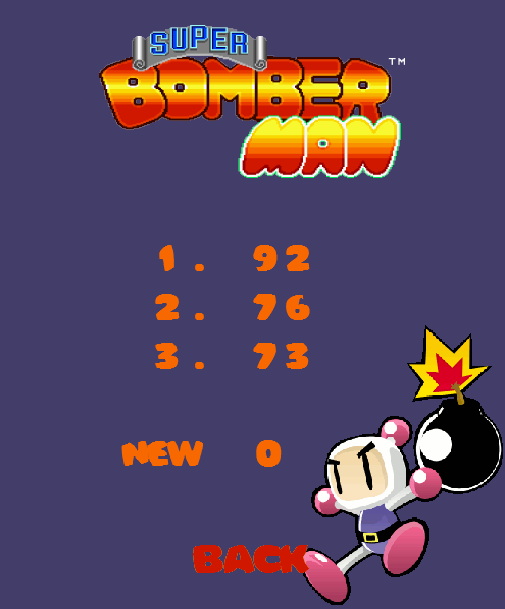
\includegraphics[width=2in]{score.png}
	\caption{Pantalla de puntuación}
	\label{fig:score}
\end{figure}
\paragraph{}Bomberman, el personaje que controla el jugador, puede moverse hacia arriba, abajo y hacia los lados; no puede atravesar bloques de ningún tipo y morirá si toca algún enemigo o la explosión de alguna bomba. Sin embargo, puede poner bombas para abrirse camino entre los bloques destruibles y eliminar los enemigos que salgan a su paso.
\paragraph{}La IA de los enemigos se ha implementado siguiendo las líneas del Bomberman clásico: patrones aleatorios de desplazamiento de los enemigos. Se ha optado por no implementar una IA más compleja ya que resultaba frustrante no poder acertarle a los enemigos y resultaba muy complicado el ganar las partidas, además de que el juego original no contaba con esa IA avanzada.
\paragraph{}Inicialmente las bombas tienen un radio de explosión de 1 casilla, sólo es posible poner una bomba a la vez en el escenario y Bomberman se mueve relativamente despacio. 
\newpage
\paragraph{}Sin embargo, conforme vaya obteniendo \textit{power ups}, el radio de las bombas cada vez es mayor, es posible poner más bombas en el escenario y Bomberman se irá moviendo más rápido, según el tipo de \textit{power up} que recoja.
\begin{figure}[H]
	\centering
	\begin{minipage}[b]{0.4\textwidth}
		\centering
		
\includegraphics[width=0.3\textwidth]{fuego.png}
		\caption{Power up que aumenta el radio de explosión de las bombas}
	\end{minipage}
	\hfill
	\begin{minipage}[b]{0.4\textwidth}
		\centering
		
\includegraphics[width=0.3\textwidth]{bomba.png}
		\caption{Power up que aumenta el número máximo de bombas en el escenario}
	\end{minipage}
	\hfill
	\begin{minipage}[b]{0.4\textwidth}
		\centering
		
\includegraphics[width=0.3\textwidth]{patines.png}
		\caption{Power up que aumenta la velocidad de Bomberman}
	\end{minipage}
	\label{fig:powerups}
\end{figure}
\paragraph{}El juego también contiene un menú principal desde el que se puede acceder a todos los apartados del mismo: 
\begin{itemize}
	\item Juego en 2D
	\item Juego en 3D
	\item Opciones de sonido
	\item Opciones de controles
	\item Ranking
	\item Créditos
\end{itemize}
\begin{figure}[H]
	\centering
	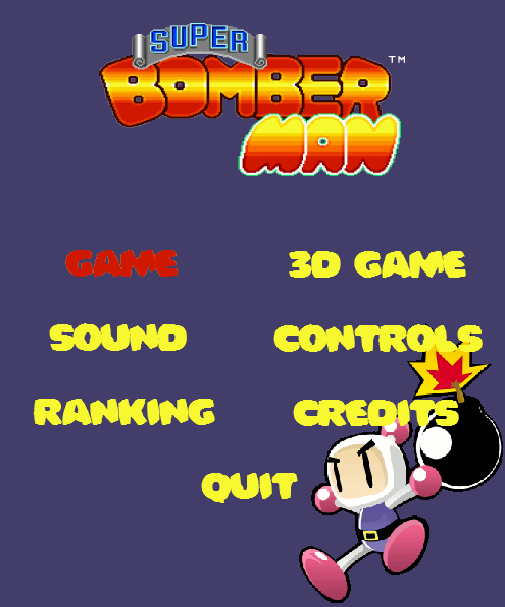
\includegraphics[width=2in]{menuses.png}
	\caption{Pantalla principal}
	\label{fig:menuses}
\end{figure}
\newpage

\section{Detalles de la implementación en 3D}
\paragraph{}En cuanto a la implementación del juego en 3D, se ha optado por utilizar una librería apta para el lenguaje Java; se trata de \textbf{libgdx}.
\paragraph{}Esta librería permite cargar modelos 3D en el juego, así como utilizar y mover una cámara por el mundo 3D. Se han utilizado modelos de cubos para los bloques, enemigos, power ups y para Bomberman, variando únicamente en el color para distinguirlos. Para las bombas y sus explosiones se han utilizado esferas y cilindros, respectivamente.
\begin{figure}[H]
	\centering
	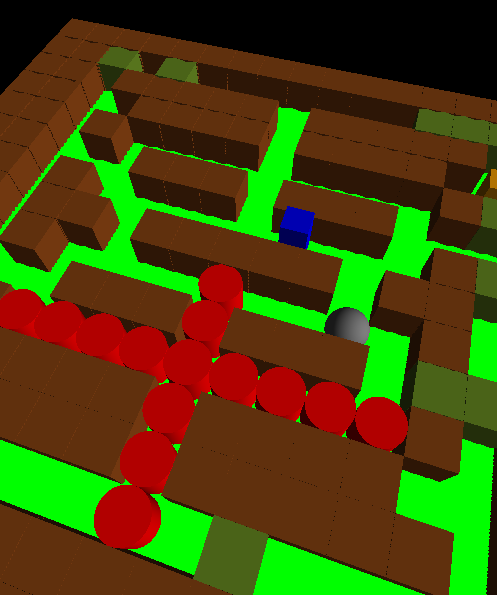
\includegraphics[width=2in]{bombermantresdes.png}
	\caption{Pantalla del juego en 3D}
	\label{fig:tresdes}
\end{figure}
Todo el sistema de juego 3D funciona exactamente igual que el 2D, únicamente cambia su aspecto visual. Sin embargo, solo se ha implementado un nivel en la versión 3D.
\newpage

\section{Principales dificultades encontradas}
\paragraph{}A continuación se describen las principales dificultades encontradas durante la realización del videojuego, todas ellas referidas a detalles técnicos. En la sección creativa no se encontraron dificultades, ya que el juego desarrollado es un clon y no un juego original.

\begin{itemize}

\item Estructura básica del juego: uno de los primeros problemas encontrados fue cómo estructurar el juego, más allá del corazón del juego. Como ambos miembros del equipo habían utilizado la herramienta GameMaker, se decidió finalmente implementar un sistema de habitaciones parecido; los objetos (las instancias que descienden de la clase Objeto) también fueron modelados de acuerdo a GameMaker, pues se consideró que era la mejor estructura que implementar.

\item El paso a 3D: para el paso a 3D del juego se decidió utilizar una librería (libgdx) ya que no se tenía tiempo suficiente para implementar un motor gráfico 3D para el juego. Esto resultó en algunos problemas, ya que solo se deseaba integrar la librería en la parte 3D del juego, y no en la 2D. Algunos de estos problemas, los más notables, fueron:

	\begin{itemize}
	\item Integración con el sistema de habitaciones realizado en el juego 2D: el juego debía funcionar igual en 3D que en 2D, y reimplementar todo para el juego 3D no era una opción. Al final, se decidió crear la habitación del juego 2D en el juego 3D, pero sin renderizarla.
	
	\item Integración con el sistema de ventanas: también hubo problemas integrando el juego 3D en el sistema de ventanas que se tenía hasta ese momento. No se pudo integrar finalmente y se tuvo que realizar el juego 3D en otra ventana aparte. Tampoco se pudo continuar el hilo del juego una vez terminado el modo 3D, ya que la librería no funcionaba bien si se recreaba la aplicación 3D más tarde.
	
	\item Cálculos en el juego: en un principio, se pensó en utilizar volúmenes envolventes para realizar el chequeo de colisiones de los cuerpos en el entorno y con otros cuerpos, pero se tuvo que desestimar la idea, ya que el cáclulo de colisiones de esta forma era muy pesado y no se podía ejecutar en el mismo hilo en el que se ejecutaba el rendering de la aplicación 3D (no había opción a ejecutarlo en otro hilo).
	\end{itemize}
	
\item El sistema de ayuda del juego: en versiones iniciales del juego no existía un sistema de ayuda al jugador para mover al Bomberman por la habitación. Esto hacía el juego muy complicado porque requería un control a nivel de píxel de las cajas de colisión, y hacía el juego muy frustrante y poco divertido. Para eliminar este problema se decidió incluir un sistema de ayuda que permite al jugador moverse más libremente: el programa rectifica la trayectoria del Bomberman para que se mueva en la dirección que el jugador desea con cierta libertad.

\item Empaquetamiento de la aplicación: al ir a empaquetar la aplicación (crear un JAR con sus contenidos) también hubo problemas y dificultades de diversas índoles que no se habían contemplado hasta ese momento en el trabajo. A continuación se explican las más importantes:

	\begin{itemize}
	\item Cambios de ruta en el JAR: al hacer el JAR el juego no funcionaba, ya que tomaba rutas relativas fuera del JAR, cuando los archivos estaban dentro. Hubo varios problemas al respecto, ya que se utilizaban tanto archivos INI como archivos de música e imágenes (stripes de sprites) y su tratamiento era diferente.
	
	\paragraph{}El principal problema era que en un JAR no hay ficheros, como en el sistema de ficheros, que es desde donde se operaba hasta ese momento, sino recursos. Para los archivos INI y las imágenes no supuso ningún problema el utilizar recursos en vez de ficheros, pero para las músicas utilizamos la librería TinySound, que requerían expresamente de ficheros. Para solucionar este contratiempo se crearon ficheros temporales en el mismo lugar donde se encontraba el JAR.
	
	\paragraph{}El segundo gran problema que surgió fue que la estructura de directorios cambió al empaquetar en un JAR, y por tanto las rutas que se utilizaban ya no eran válidas. Para ello hubo que cambiar las rutas para que fueran relativas desde dentro de la carpeta ''resources''.
	
	\item Lentitud al cargar el JAR: en un principio se decidió empaquetar las librerías utilizadas dentro del JAR creado, pero debido a esto el juego cargaba muy lento desde el JAR (podía llegar a tardar un minuto en salir de la pantalla de carga, cuando desde el sistema de ficheros el juego tardaba menos de diez segundos en cargar).
	
	\paragraph{}Después de investigar este problema, el equipo se dio cuenta de que el empaquetamiento de librerías en el JAR era el causante de la lentitud. Como las librerías estaban empaquetadas, el JAR debía extraerlas y verificarlas cada vez que se lanzaba, y la etapa de verificación era muy costosa.
	
	\paragraph{}La solución a este problema fue tan sencilla como extraer las librerías dentro del JAR.
	\end{itemize}

\end{itemize}
\newpage

\section{Módulos y paquetes del juego}

\subsection{Librerías utilizadas}

\paragraph{}A continuación se listan las librerías externas que se han utilizado en la elaboración del juego y qué trabajos desarrollan dichas librerías dentro del juego.

\begin{itemize}
\item TinySound: es la librería responsable de reproducir la música de fondo y efectos de sonidos dentro del juego.

\item Ini4j: es la librería encargada del acceso a los archivos INI. Proporciona una interfaz amigable para el acceso a archivos de este tipo y aunque este trabajo podría haberlo hecho el equipo sin una carga de trabajo adicional considerable, se decidió apoyarse en esta librería por la simplicidad de su API.

\item Libgdx: es la librería encargada de gestionar la parte 3D del juego; es decir, es el motor gráfico 3D del juego.
\end{itemize}
\newpage

\section{Reparto de tareas}

\paragraph{}A continuación se muestra el reparto de tareas de acuerdo a los grandes bloques del juego. No obstante, los dos miembros del equipo han participado en todas las tareas; este reparto muestra quién ha realizado más en la tarea, y no es exclusiva de una persona.

\begin{itemize}
\item Estructura básica del juego: Jaime Ruiz-Borau.
\item Inteligencia Artificial: Patricia Lázaro.
\item Control del personaje: Jaime Ruiz-Borau y Patricia Lázaro.
\item Menús: Jaime Ruiz-Borau y Patricia Lázaro.
\item Música: Jaime Ruiz-Borau.
\item Gráficos: Jaime Ruiz-Borau y Patricia Lázaro.
\item Paso a 3D: Patricia Lázaro.
\end{itemize}
\newpage

\begin{thebibliography}{99}
	\bibitem{fig:primerBomberman} \textbf{Imágenes del primer Bomberman} - By Source, Fair use, [\url{https://en.wikipedia.org/w/index.php?curid=12465479}]
	
	\bibitem{} \textbf{Enlace al repositorio de Github} - [\url{https://github.com/EquipoJP/SuperBomberman}]
	
	\bibitem{} \textbf{Descargas del juego} - [\url{https://github.com/EquipoJP/SuperBomberman/releases}]
	
	\bibitem{} \textbf{Página principal de Ini4j} - [\url{http://ini4j.sourceforge.net/}]
	
	\bibitem{} \textbf{Página principal de TinySound} - [\url{https://github.com/finnkuusisto/TinySound}]
	
	\bibitem{} \textbf{Página principal de Libgdx} - [\url{https://libgdx.badlogicgames.com/}]
	
\end{thebibliography}

\end{document}